\chapter{Dynamic analysis}

\section{Legend}
	\begin{figure}[ht]
			\begin{center}
				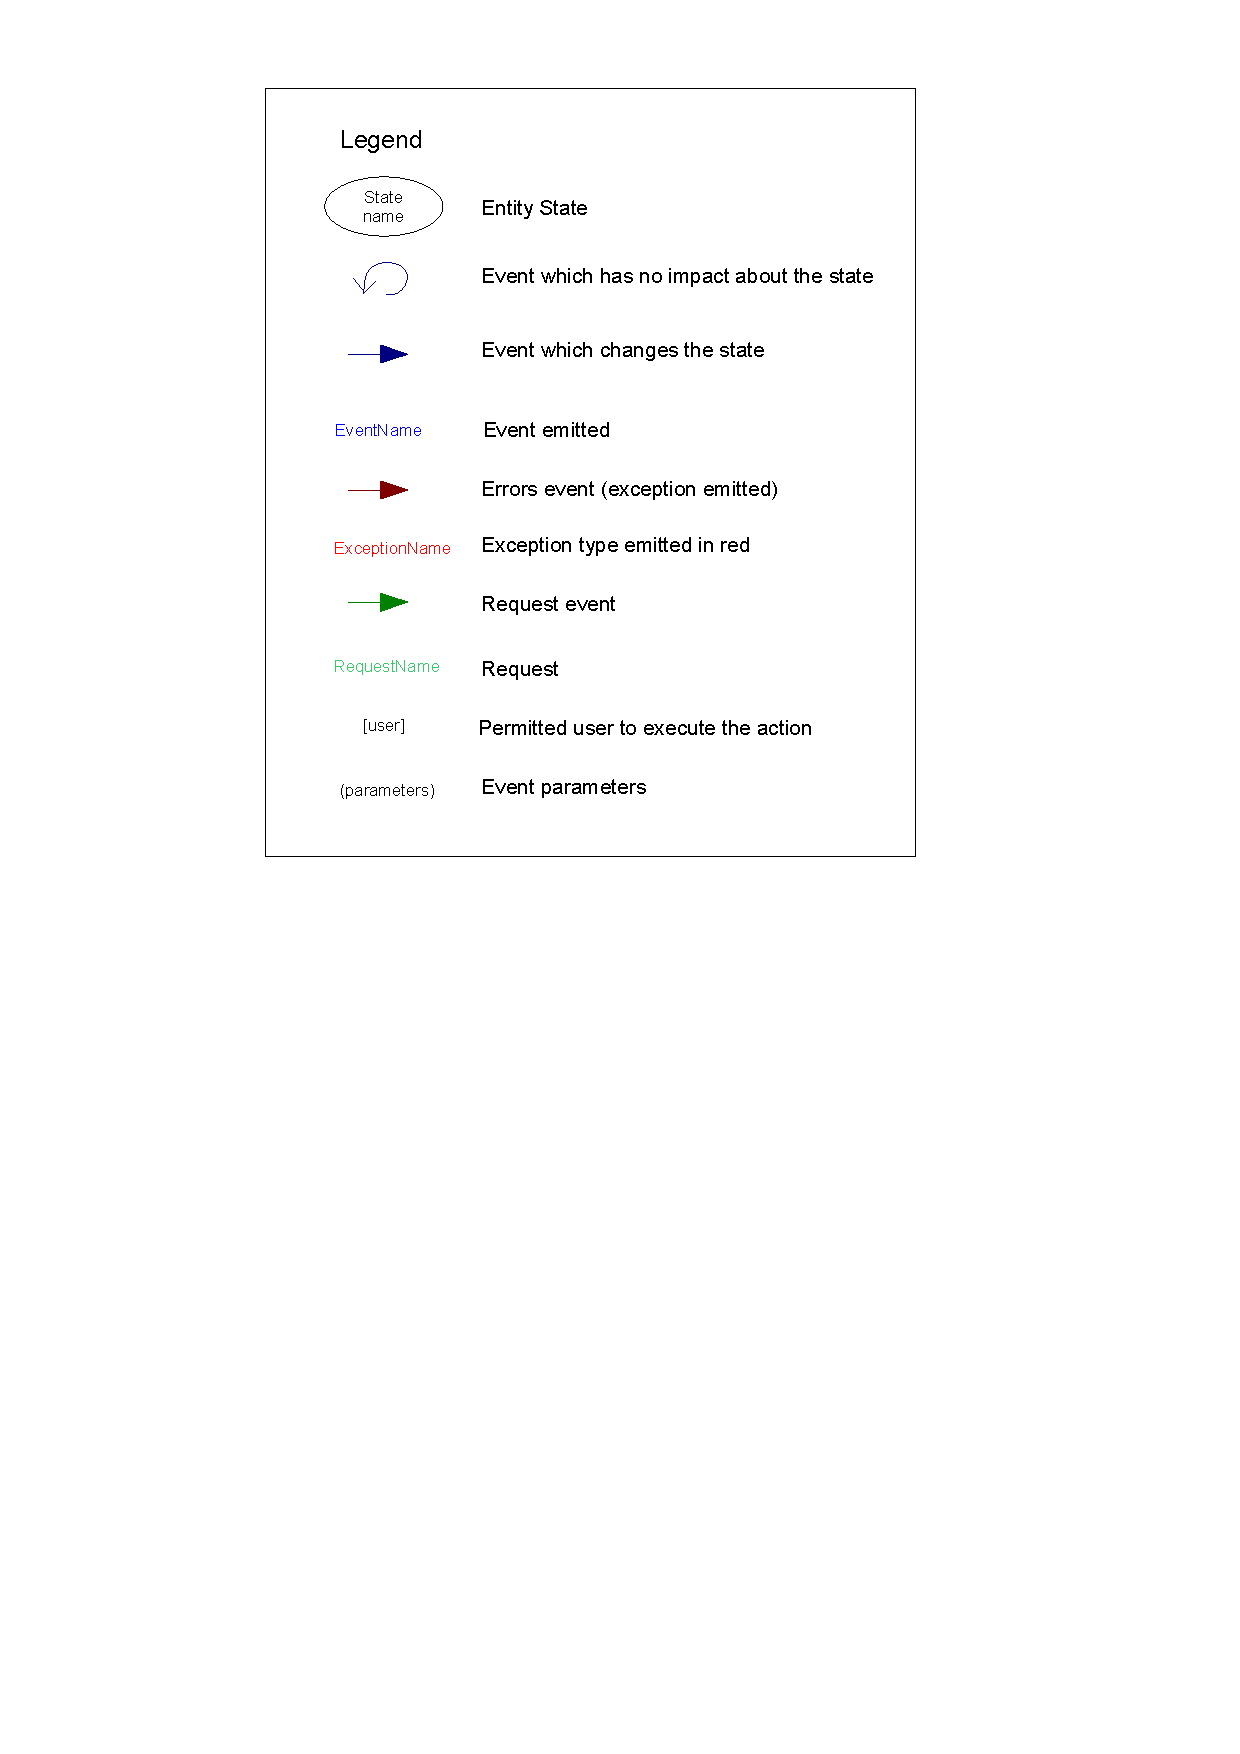
\includegraphics[width=\textwidth,  trim=2cm 14cm 2cm 1cm]{UML_figure/state_transition/dojo_logic/st_legend.pdf}
				\caption{Legend for state transition diagram}
			\end{center}
	\end{figure}
\newpage
\section{User}
	\begin{figure}[ht]
			\begin{center}
				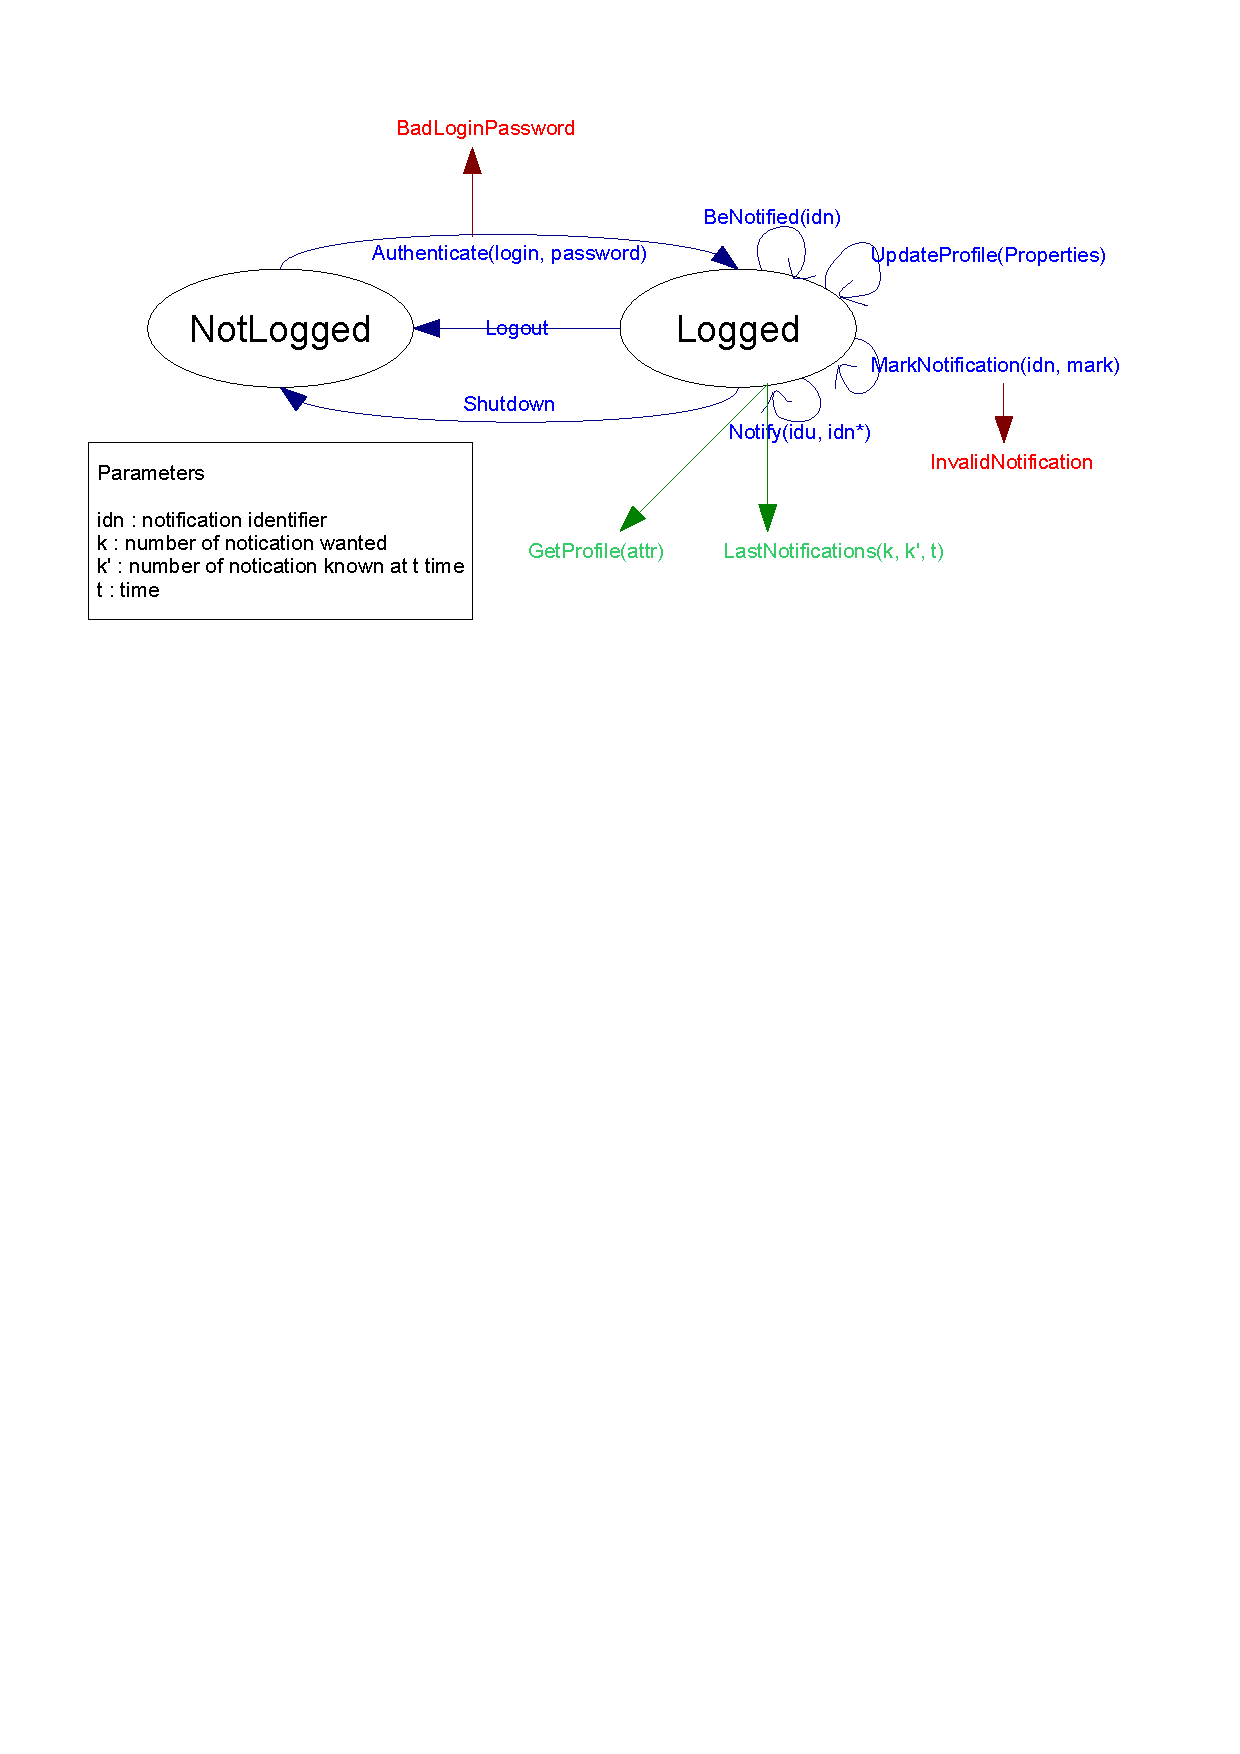
\includegraphics[width=\textwidth,  trim=2cm 17cm 2cm 1cm]{UML_figure/state_transition/dojo_logic/st_user.pdf}
				\caption{User state transition diagram}
			\end{center}
	\end{figure}
	\subsection{States}
		\subsubsection{Not logged}
			This state represents the fact that a user is not logged. This is a unidentified user.
		\subsubsection{Logged}
			This state represents the fact that a user is logged. This is an identified user.
	\subsection{Event : state modifier}
		\subsubsection{Authenticate}
			This event triggered by an unidentified user. It can produce error when the login and password does not match with any registered user.
		\subsubsection{Logout}
			This event asked by an identified user to log out.
		\subsubsection{Down}
			This event pushes by the system to log out all identified users.
	\subsection{Event : state keeper}
		\subsubsection{Be notified}
			This event notifies a logged user for new messages.
		\subsubsection{UpdateProfile}	
			This event updates the profile of logged user with new properties.
		\subsubsection{Mark Notification}
			This event marks a notification as received. It can produce error when the notification does not exist.
		\subsubsection{Notify}
			This event pushes by a registered user to send a notification to other registered user.
	\subsection{Request}
		\subsubsection{GetProfile}
			This request retrieves user data profile.
		\subsubsection{LastNotification}
			This request retrieves last notifications since time t and k the number of wanted notifications.
	\subsection{Errors}
		\subsubsection{BadLoginPassword}
			This error is thrown when the login or the password is incorrect.
\newpage
\section{Group}
	\begin{figure}[ht]
			\begin{center}
				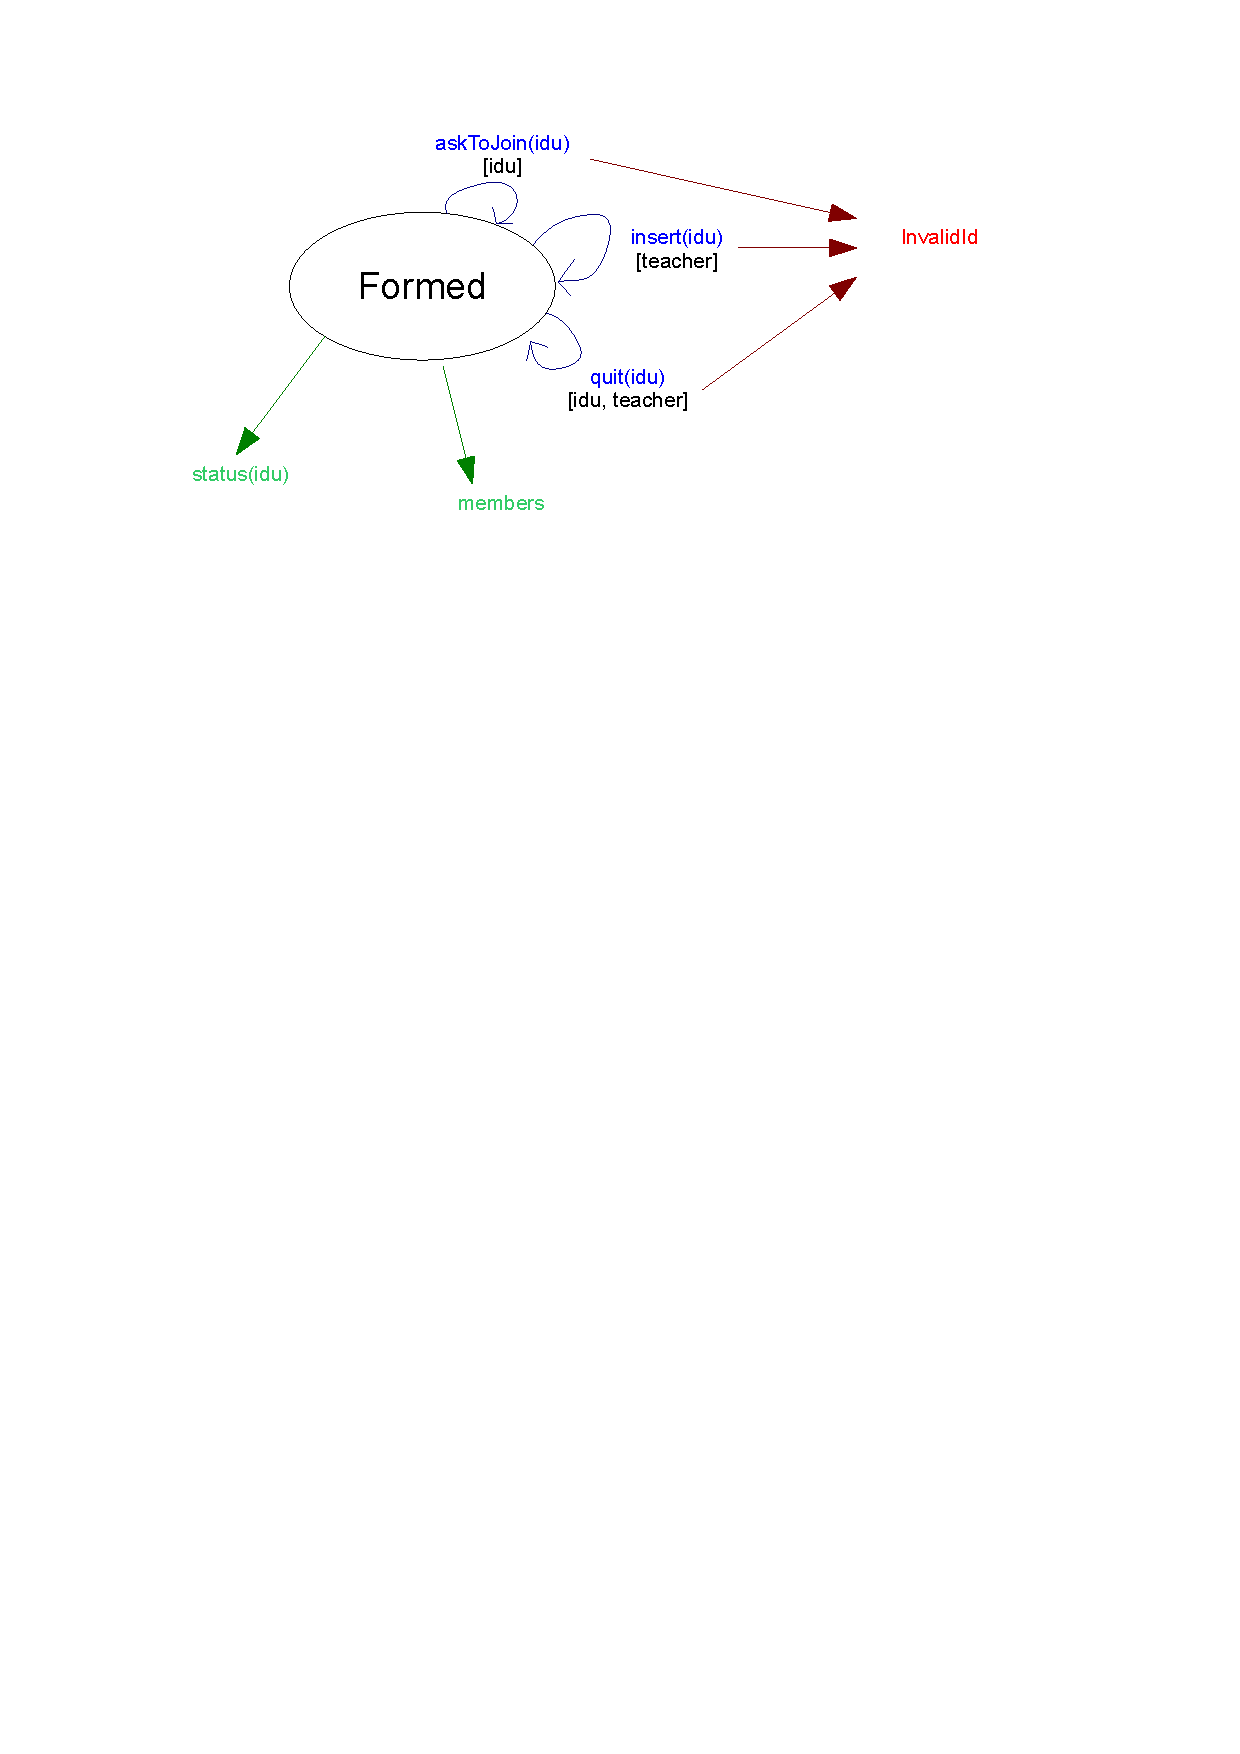
\includegraphics[width=\textwidth,  trim=2cm 18cm 2cm 1cm]{UML_figure/state_transition/dojo_logic/st_group.pdf}
				\caption{Group state transition diagram}
			\end{center}
	\end{figure}
	\subsection{States}
		\subsubsection{Formed}
			This state represents a formed group.
	\subsection{Event : state keeper}
		\subsubsection{AskToJoin}
			This event triggered by an identified user to join the group, can produce error when the user is already undefined.
		\subsubsection{Insert}
			This event inserts an identified user to the group, only used by teacher user.
		\subsubsection{Quit}
			This event formulated by a member from the group or a teacher to leave the group.
	\subsection{Request}
		\subsubsection{Status}
			This request retrieves the status of each members.
		\subsubsection{Members}
			This request retrieves the group members.
	\subsection{Errors}
		\subsubsection{InvalidId}
			This error is thrown when the user cannot execute these events.
\newpage
\section{Exercise}
	\begin{figure}[ht]
			\begin{center}
				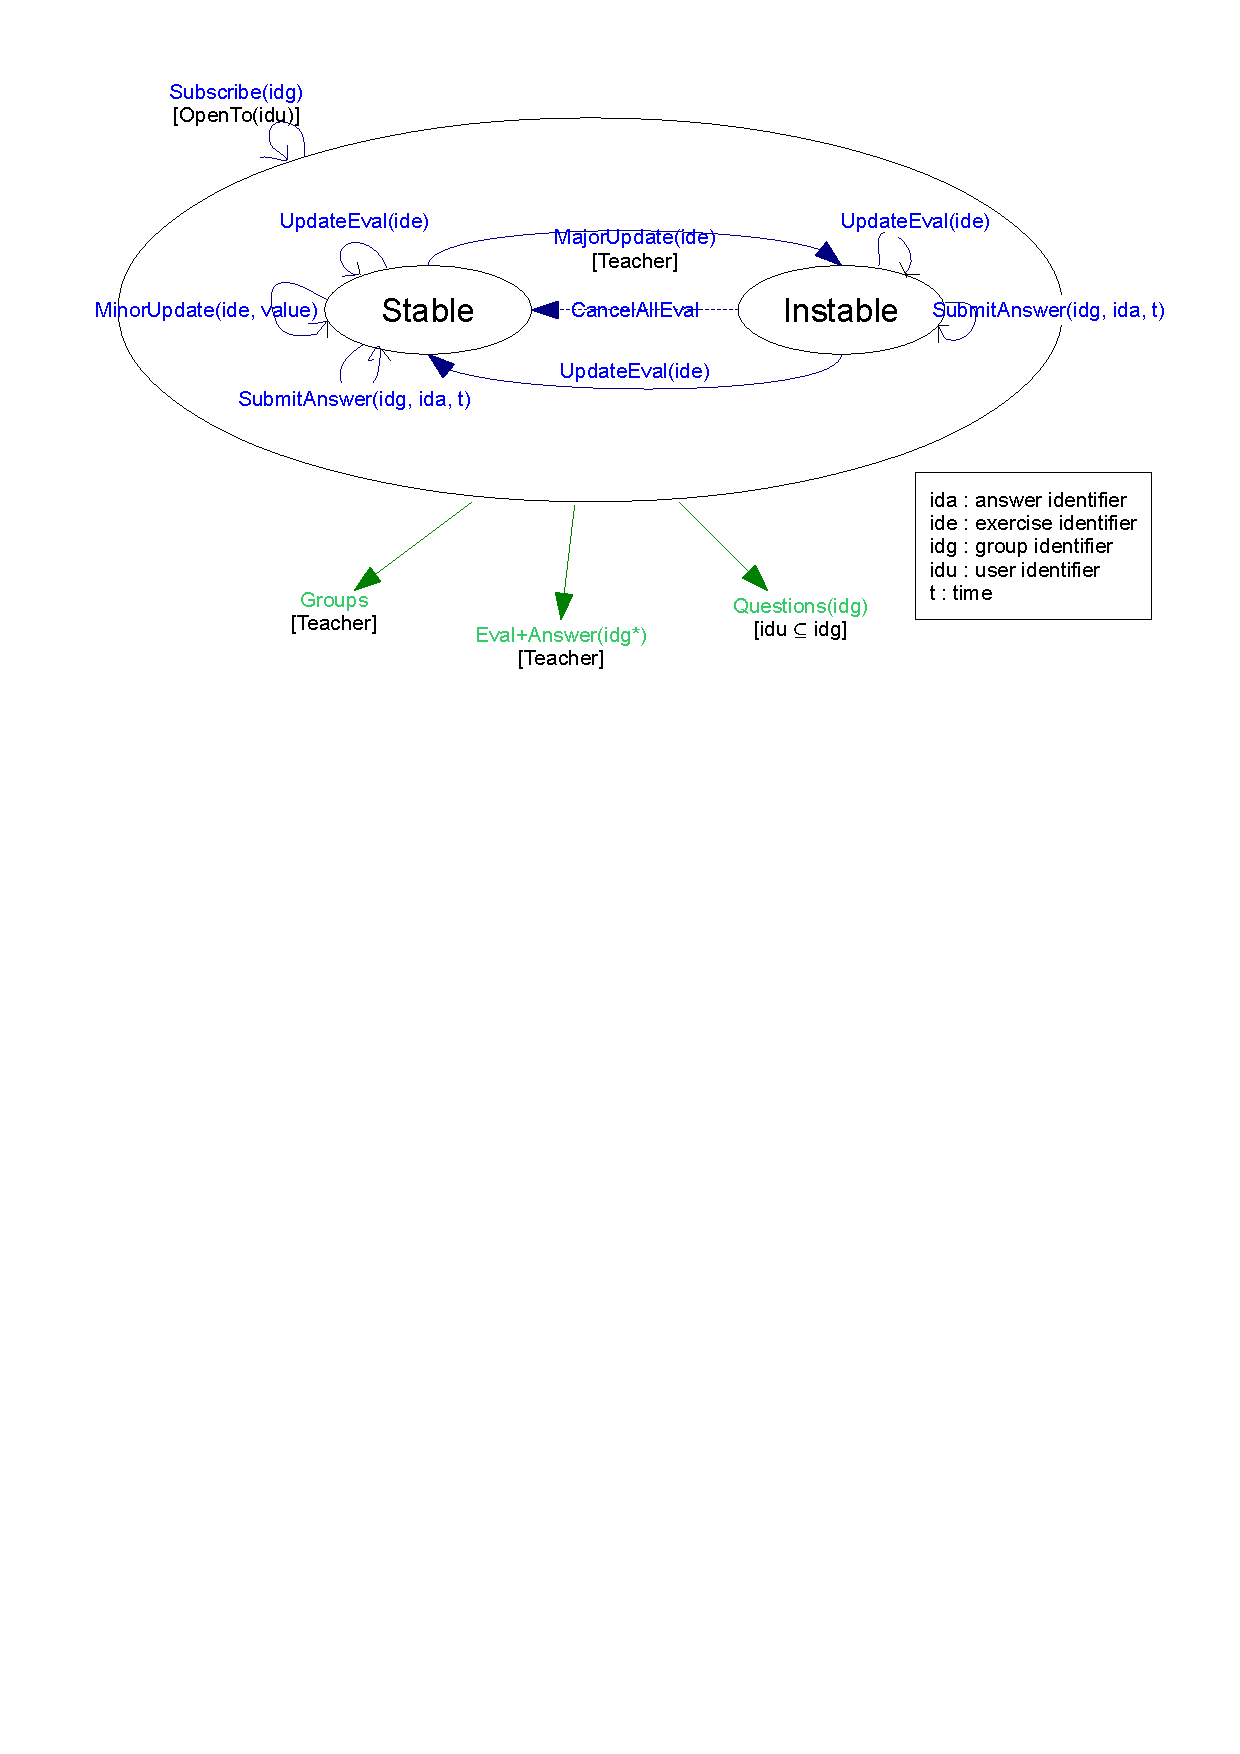
\includegraphics[width=\textwidth,  trim=2cm 18cm 2cm 1cm]{UML_figure/state_transition/dojo_logic/st_exercise.pdf}
				\caption{Exercise state transition diagram}
			\end{center}
	\end{figure}
	\subsection{States}
		\subsubsection{Stable}
			This state represents the stable version of an exercise, the exercise correction has not changed meaning the evaluation system has not changed.
		\subsubsection{Unstable}
			This state represents an exercise which undergoes a major update, the exercise correction is altered with the evaluation system.\\
			At this point, some running evaluation might be inconsistent with respect to the new grading system.
	\subsection{Event : state modifier}
		\subsubsection{MajorUpdate}
			This event is called when the evaluation method for an exercise has to change, for instance changing a coding question by a free question.
		\subsubsection{CancelAllEval}
			This event is called by the platform or the administrator meaning that all exercises which being evaluated have to be cancelled.
		\subsubsection{UpdateEval}
			This event is called when there is no more running evaluation in an inconsistent state.
	\subsection{Event : state keeper}
		\subsubsection{UpdateEval}
			This event is called when an evaluation is running in an inconsistent state.
		\subsubsection{MinorUpdate} 	
			This event is called when the teacher does a minor update for an exercise.
			A minor update is an update which does not affect the grading system.
		\subsubsection{SubmitAnswer}
			This event is called when an answer is submitted and has to be evaluated.
	\subsection{Request}
		\subsubsection{Groups}
			This request retrieves the list of groups that have subscribed to this exercise.
		\subsubsection{Eval+Answer}
			This request retrieves evaluation and answer for a group subscribed to this exercise.
		\subsubsection{Questions}
			This request retrieves questions from the exercise for a specific group.
\newpage
\section{Answers}
	\begin{figure}[ht]
			\begin{center}
				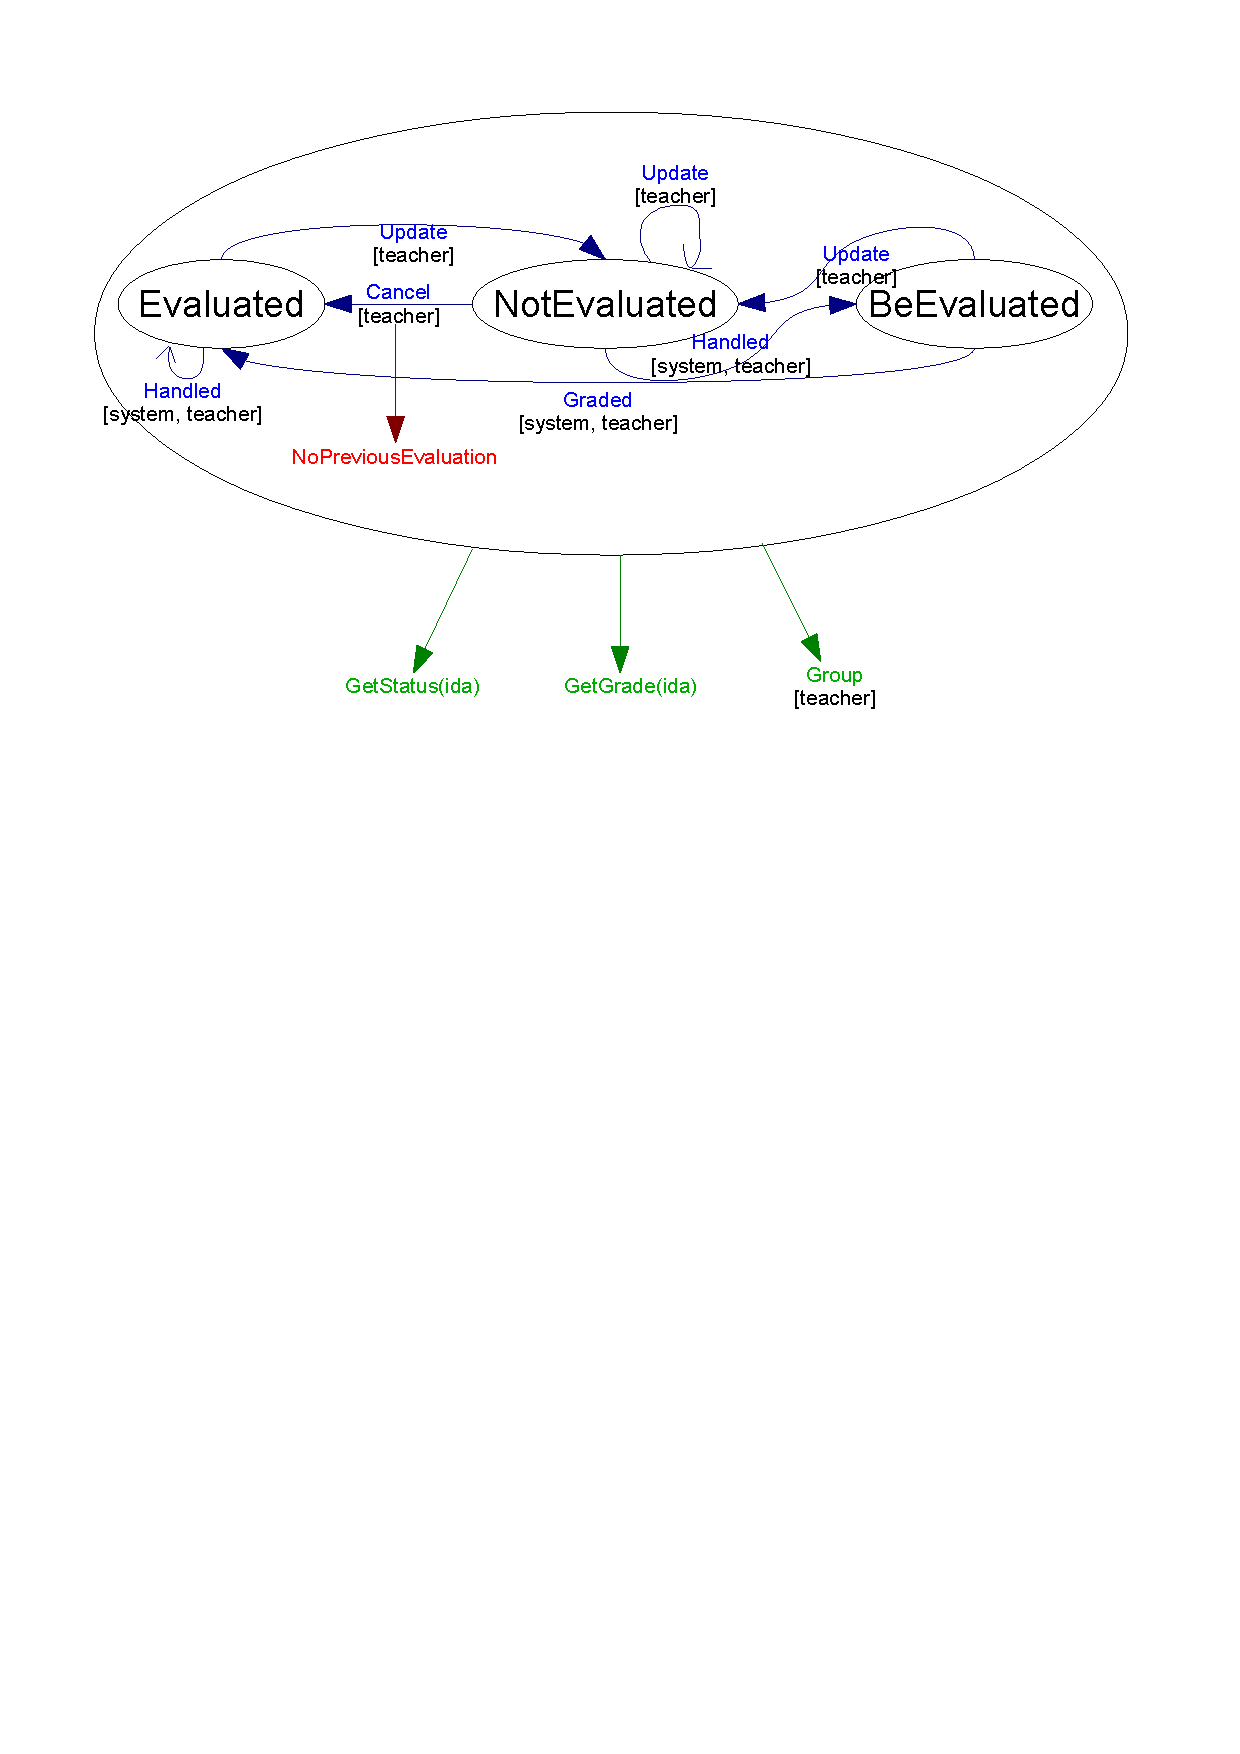
\includegraphics[width=\textwidth,  trim=2cm 16cm 2cm 1cm]{UML_figure/state_transition/dojo_logic/st_answers.pdf}
				\caption{Answers state transition diagram}
			\end{center}
	\end{figure}
	\subsection{States}
		\subsubsection{Evaluated}
			This states represents an answers entity which is already graded according to the evaluations entity associated.
		\subsubsection{Not Evaluated}
			This state represents an answers entity which is not yet graded or the grade does not match with the current evaluations entity associated
		\subsubsection{Be Evaluated}
			This state represents an answers entity which is under an evaluation.
	\subsection{Event : state modifier}
		\subsubsection{Update}
			This event is called when the teacher makes update. 
		\subsubsection{Graded}
			This event is called when the grade system has finished to handle a non evaluated answers.
		\subsubsection{Handled}		
			This event is called when a non evaluated answers need to be graded.
		\subsubsection{Cancel}
			This event is called when a teacher decide to keep a previous graded answers, then to not take in account the new evaluations.
	\subsection{Event : state keeper}
		\subsubsection{Handled}
			This event is called when an already graded answers entity try to be graded again.
		\subsubsection{Update}
			This event is called when a teacher updates the answers.
	\subsection{Request}
		\subsubsection{Group}
			This request retrieves the group information of this answers entity.
		\subsubsection{Get Status}
			This request retrieves the state associate to the answers identifier.
		\subsubsection{Get Grade}
			This request retrieves the grade associate to the answers identifier.
	\subsection{Errors}
		\subsubsection{NoPreviousEvaluation}	
			This error is thrown when an answers entity does not have any previous evaluated state.
\newpage
\section{Evaluations}
	\begin{figure}[ht]
			\begin{center}
				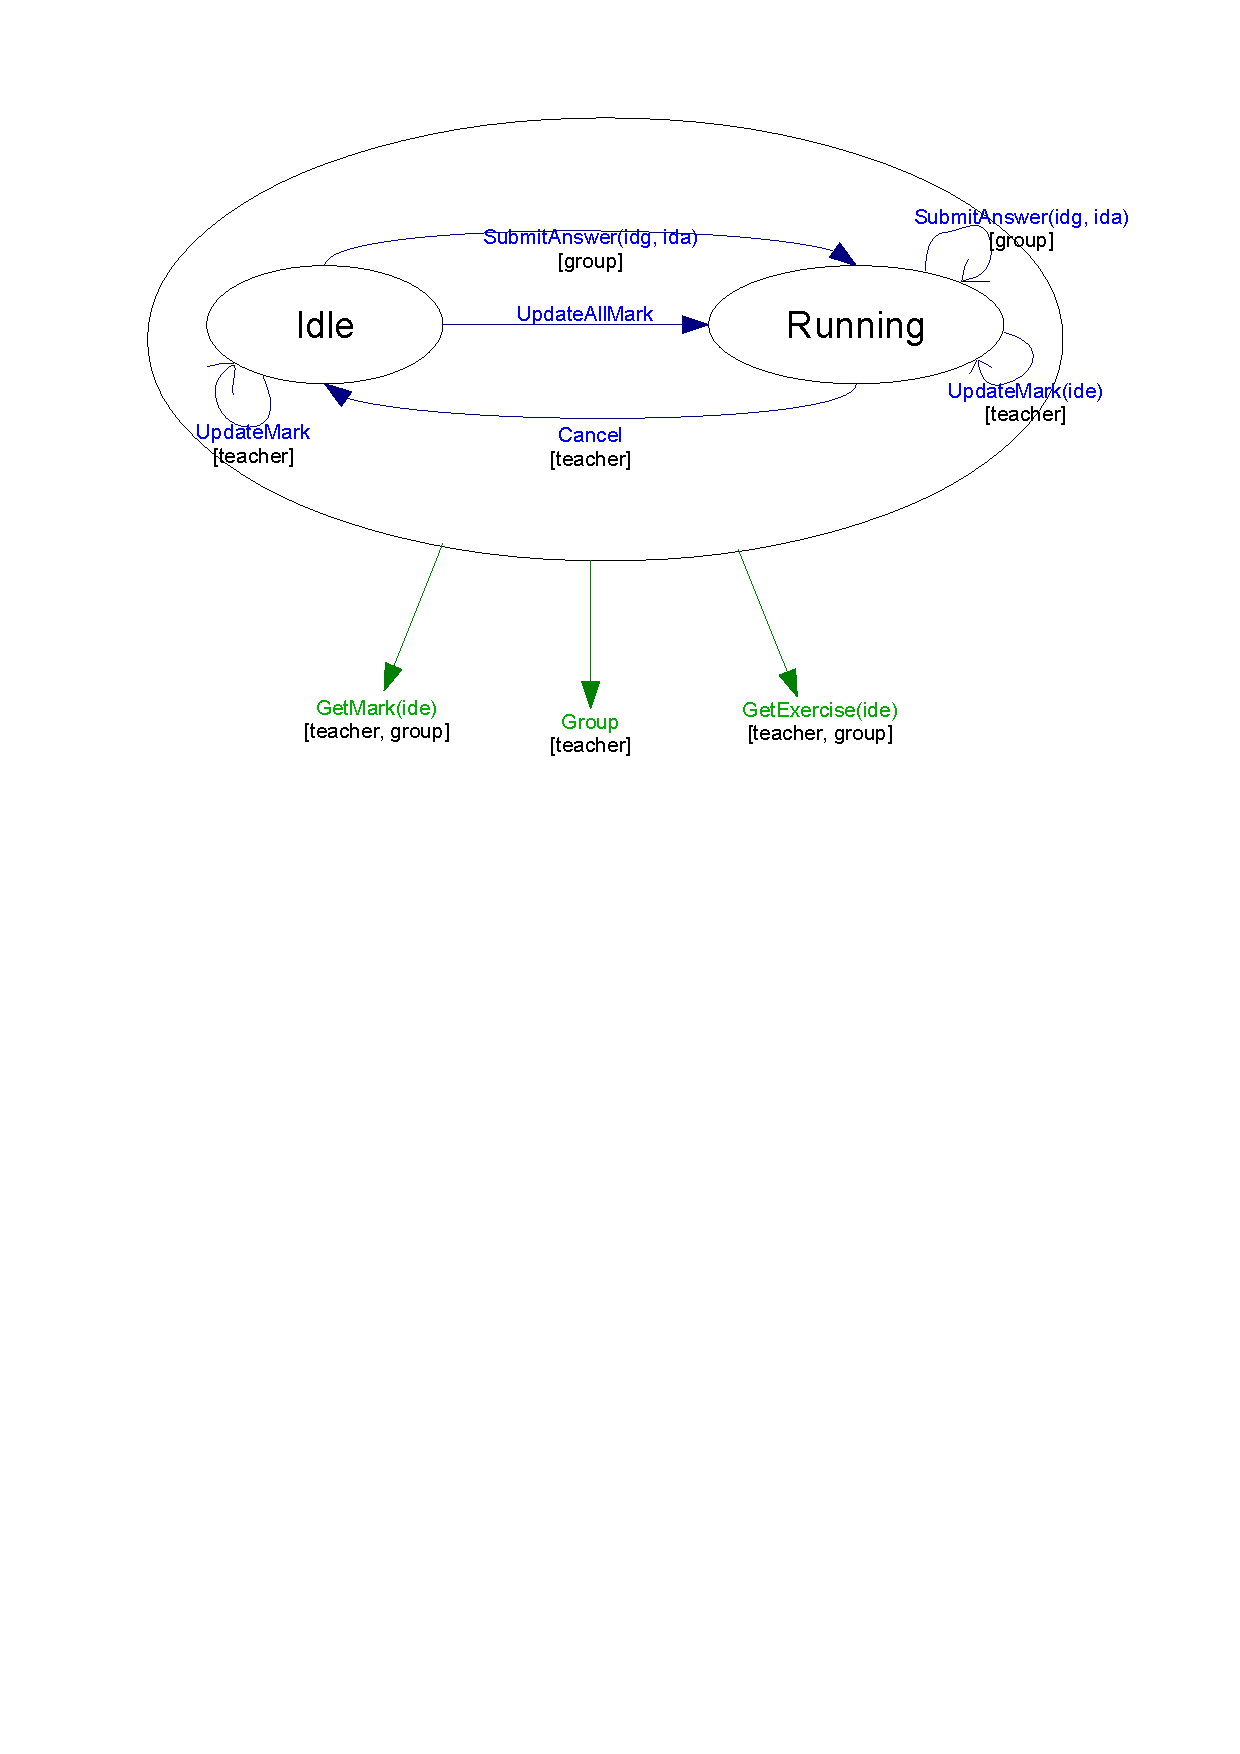
\includegraphics[width=\textwidth,  trim=2cm 16cm 2cm 1cm]{UML_figure/state_transition/dojo_logic/st_evaluations.pdf}
				\caption{Evaluations state transition diagram}
			\end{center}
	\end{figure}
	\subsection{States}
		\subsubsection{Idle}
			This state represents a finished evaluation.
		\subsubsection{Running}
			This state represents an evaluation in progress.
	\subsection{Event : state modifier}
		\subsubsection{SubmitAnswer}
			This event is called when answers are submitted and have to be evaluated.
		\subsubsection{UpdateAllMark}
			This event is called when the teacher has changed the evaluation system and answers are submitted.
		\subsubsection{Cancel}
			This event is called when the teacher wants to cancel a running evaluation.
	\subsection{Event : state keeper}
		\subsubsection{UpdateMark : Idle}
			This event is called when the teacher updates the evaluation system and no answers are submitted.
		\subsubsection{UpdateMark : Running}
			This event is called when the teacher updates the evaluation system and an evaluation is running.
		\subsubsection{SubmitAnswer}
			This event is called when a group submit new answers and the evaluation associated is running.
	\subsection{Request}
		\subsubsection{Group}
			This request retrieves the group information associated to the evaluation.
		\subsubsection{GetMark}
			This request retrieves the mark associated to the exercise.
		\subsubsection{GetExercise}
			This request retrieves the exercise associated to the evaluation.
			
			
	
			


